\errorcontextlines 999999
\PassOptionsToPackage{table}{xcolor}
\PassOptionsToPackage{defernumbers=true}{biblatex}
\documentclass[aspectratio=169,usepdftitle=true,11pt,fleqn,english,c]{beamer}

\usepackage{babel}

\usepackage[%
    sopra-listings={encoding,cpalette,fakeminted,highlights},%
    sopra-tables, color-palettes={addons},%
    lecture-bibliography={biber,style=numeric-comp},%
    util, lithie-boxes={germanenv,koma,overwrite},%
    lithie-task-boxes={cpalette}, lecture-links={patchurl},%
    lecture-registers={disable}% would interfere with beamer
]{lithie-util}

\solLoadLanguage{bash,javascript}
\makeatletter
\sol@list@define@styles{%
  {keywordA: \@declaredcolor{sol@colors@lst@keywordA}\bfseries},%
}
\makeatother

\RestyleAlgo{plain}
\lstset{lineskip=5.5pt}
\lstfs{10}

\DefinePalette{Rekursion}
{Red,rötlich: RGB(93, 46, 70)}
{Blau,bläulich: RGB(22, 105, 122)}
{Lila,lilafarben: RGB(93, 45, 108)}
{Grün,grünlich: RGB(21, 150, 90)}
\SetShadeContrast{45}
\UsePalette{Rekursion}

\usetheme[libs,nofootfade,centerfoot]{dividing-lines}
\SetColorProfile*{paletteA}{paletteB}{paletteC}

\usetikzlibrary{arrows.meta,decorations,tikzmark,matrix,decorations.pathmorphing, decorations.pathreplacing, decorations.shapes}
\def\info#1{\bgroup\scriptsize\textcolor{gray}{(#1)}\egroup}
\SetAllLinkStyle{#1}
\def\fillfont{\def\mdseries@sf{medium}\sffamily}
\colorlet{lgray}{lightgray!48!white}

\usepackage[glows]{tikzpingus}
\usetikzlibrary{decorations.text,graphs}
\hypersetup{colorlinks=false}
\def\rhead#1{\hfill\textcolor{shadeA}{\sbfamily#1}}

\newsavebox\parallellogo
\setbox\parallellogo=\hbox{\tikzpicture[xscale=1.25] % stretch me
\foreach[count=\y from 0] \line in {0,.25,.5,.25,0,.25,.5,.25,0} {
\scope[shift={(\line,-\y)}]
  \foreach\i in {1,3,...,14} {
    \fill (\i,0) rectangle ++(1,1);
    % bars
    \draw[gray,very thick] (\i,0) -- ++(0,1) (\i+1,0) -- ++(0,1);
  }
  \draw[gray,very thick] (0,0) rectangle ++(15,1);
\endscope
}
\endtikzpicture}
% no depth!
\title{\texorpdfstring{\smash{\resizebox*!{\ht\strutbox}{\copy\parallellogo}}~}{}GNU parallel}
\subtitle{Parallelizing and\texorpdfstring{\\}{\space}Distributing programs with the Shell}
\institute{\textsc{ccpdp}, Universität Ulm}

\author[Felix R. \& Florian S.]{Felix Rieg and Florian Sihler}
\email{florian.sihler@uni-ulm.de}

\date{\today}
\outro{Ulm, \today}
\license[]{All rights reserved}

\colorlet{codeouthl}{gray!42!white}

\newsavebox\titleimg
\setbox\titleimg=\hbox{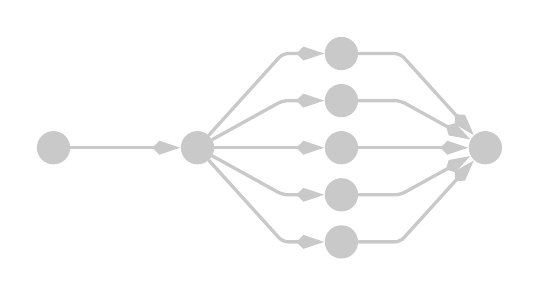
\begin{tikzpicture}[codeouthl]
  \matrix[matrix of nodes,nodes={circle,fill},above right,ampersand replacement=\&,column sep=4em,row sep=.5em] {
           \&        \& |(3a)|~ \&        \\
           \&        \& |(3b)|~ \&        \\
    |(1)|~ \& |(2)|~ \& |(3c)|~ \& |(4)|~ \\
           \&        \& |(3d)|~ \&        \\
           \&        \& |(3e)|~ \&        \\
  };
  % wellp: c\graph[edges={very thick,-Kite}]{(1) -> (2) -> {(3a),(3b),(3c),(3d),(3e)} -> (4)};
  \scope[every path/.append style={draw,very thick,-Kite,rounded corners=2pt,line cap=round}]
  \path(1) -- (2);  \path(2) -- (3c); \path(3c) -- (4);
  \foreach\a in {a,b,d,e} {
    \path (2) -- ([xshift=-1.5em]3\a.west) -- (3\a.west);
    \path (3\a.east) -- ++(1.5em,0) -- (4);
  }
  \endscope
\end{tikzpicture}}
\def\PostTitlepage{\begin{tikzpicture}[overlay,remember picture]
\node[above right=.5cm,xshift=1cm,scale=.875] at(current page.south west) {\copy\titleimg};
\end{tikzpicture}}

\addbibresource{./references.bib}

\makeatletter
\newcommand*\md{\@ifstar{\@md}{\@md{0}}}% with star we can set handout state
\def\@md#1#2{\only<#2|handout:#1>{\llap{\color{shadeA}\textbullet~}}}
\newcommand*\mb[2][0]{\only<#2|handout:#1>{\rlap{\smash{\raisebox{-.66\baselineskip}{\color{shadeA}\textbullet}}}}}
\newcommand*\mh[2][0]{\only<#2|handout:#1>{\color{shadeA}\textbullet}}
\newcommand*\mdl[2][0]{\only<#2|handout:#1>{\llap{\smash{\raisebox{-.5\baselineskip}{\tikz{\fill[shadeA,rounded corners=1pt] (0,-.65mm) rectangle ++(2.15\p@,\baselineskip+.65mm);}}~}}}}
\makeatother


\setcounter{tocdepth}{4}
\newsavebox\pinguA \newsavebox\pinguB \newsavebox\pinguC

\usepackage[link]{qrcode}
% TODO
\outroright{% \smash{\raisebox{1.33cm/2}{
% \qrcode[height=1.33cm]{https://github.com/EagleoutIce/Episode-Recursion}}}\begin{tikzpicture}[remember picture,overlay]
% \node[above left,btdl@color@white,scale=.475] at (current page.south east) {\href{https://github.com/EagleoutIce/Episode-Recursion}{Slides and \LaTeX-sources on GitHub!}};
% \end{tikzpicture}
}

\long\def\commy#1{\smash{\tiny\fboxsep=1pt\fcolorbox{pingu@purple}{pingu@purple!10!white}{\bfseries #1}}}
\long\def\flo#1{\commy{Flo:~#1}}
\long\def\felix#1{\commy{Felix:~#1}}

\usepackage{xspace}
\def\LogoParallel{parallel\xspace}%{para\textit{ll}\/el\xspace}
\makeatletter
\def\sol@minted@setup#1#2#3{\lstset{style=#1,language=#2,lineskip=4pt,#3,escapeinside={/*}{*/}}}
\solsetmintedstyle{plain}% number}

\def\HStrut{\vphantom{\{\}g}}
% we do not nest inside tikzmarknode as this is not possible
\def\Snode#1{\tikzmarknode{#1}\HStrut}
\def\bnode#1#2{\rnode{#1}{\sbasic{#2}}}%
\def\rnode#1#2{\Snode{#1}#2\Snode{#1@}}
\def\CodeFileMarker#1{{\color{gray}\sffamily\fontseries{l}\tiny\llap{\faFileCodeO~\thinspace}#1}}
